\documentclass[tikz,border=3.14mm]{standalone}
\usepackage{pgfplots}
\pgfplotsset{compat=1.18}

\begin{document}
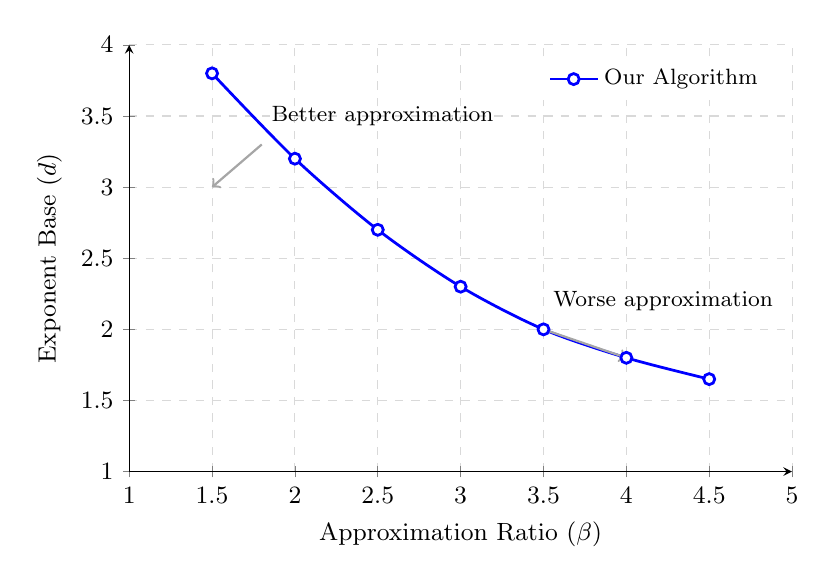
\begin{tikzpicture}
\begin{axis}[
    width=10cm,
    height=7cm,
    axis lines=left,
    xlabel={Approximation Ratio ($\beta$)},
    ylabel={Exponent Base ($d$)},
    xmin=1, xmax=5,
    ymin=1, ymax=4,
    grid=both,
    grid style={dashed, gray!30},
    xtick={1,1.5,2,2.5,3,3.5,4,4.5,5},
    ytick={1,1.5,2,2.5,3,3.5,4},
    tick label style={font=\small},
    label style={font=\small},
    legend style={
        at={(0.97,0.97)},
        anchor=north east,
        font=\footnotesize,
        draw=none
    },
    mark options={solid, scale=1.2}
]

% Theoretical curve (hypothetical relationship)
\addplot[
    smooth,
    color=blue,
    line width=1pt,
    mark=*,
    mark options={fill=white}
] coordinates {
    (1.5, 3.8)
    (2.0, 3.2)
    (2.5, 2.7)
    (3.0, 2.3)
    (3.5, 2.0)
    (4.0, 1.8)
    (4.5, 1.65)
};
\addlegendentry{Our Algorithm}

% Annotations
\node[anchor=west, font=\footnotesize] at (axis cs:1.8,3.5) {Better approximation};
\node[anchor=west, font=\footnotesize] at (axis cs:3.5,2.2) {Worse approximation};
\draw[->, thick, gray!70] (axis cs:1.8,3.3) -- (axis cs:1.5,3.0);
\draw[->, thick, gray!70] (axis cs:3.5,2.0) -- (axis cs:4.0,1.8);

\end{axis}
\end{tikzpicture}
\end{document}